\documentclass{beamer}
\usepackage[utf8]{inputenc}
\usepackage[T1]{fontenc}
%\usepackage[french]{babel}
\usepackage{amsmath, amsfonts, amsthm, amssymb}
\usepackage{hyperref}
\usepackage{tcolorbox}

\newtheorem{exo}{Exercise}

\title{GIT tutorial}
\author{Pauline Hubert and Nadia Lafrenière}
\date{FPSAC software days, July 2019}
\begin{document}
	\maketitle
	\begin{frame}{Motivation}
		Dossier de Duncan
		\pause
		PhD Comics
		\pause
		Long échange de courriels
	\end{frame}
	\begin{frame}{What software to use? Pros and cons}
		\begin{tabular}{lp{0.35\linewidth}p{0.35\linewidth}}
%			\hline
			& Pros & Cons\\
			\hline
			Email & "Easy" to use & So many!\\
			\hline
			Overleaf & Many people can work at the same time & Only online, latex only\\
			\hline
			Dropbox & Easy to use & No two people can work at the same time, no version control\\
			\hline
			Git & Version control, automatic fusion of modifications, any file type & More difficult to start\\
%			\hline
		\end{tabular}
	\end{frame}
	\begin{frame}{What is Git?}
		Git is a version control software. \newline
		
		\begin{itemize}
			\item It keeps track of every modifications.
			\item You can go back in time to a previous version.
			\item It allows many people to work in parallel.
		\end{itemize}	
	\end{frame}
	\begin{frame}{Online servers for Git}
		Store your data somewhere. \newline 
			\begin{itemize}
				\item Local : on your computer.
				\item Online servers : Github, Bitbucket, GitLab, University server, etc. \newline
			\end{itemize}
		If you use an online server, you will also have a local version on your computer. If you want to work with other people, you have to use a server. 
	\end{frame}
	\begin{frame}{Now that you are convinced... Installation}
		\begin{itemize}
			\item Linux : Type in shell \texttt{sudo apt install git}
			\item MacOS : Go to \url{git-scm.com/download/mac}
			\item Windows : Go to \url{gitforwindows.com}
		\end{itemize}
	\end{frame}
	\begin{frame}[fragile]{Configuration}
	To share code, you need to identify yourself:
	\begin{verbatim}
$ git config --global user.name "John Doe"
$ git config --global user.email "john.doe@email.com"
	\end{verbatim}
	Please, do not use this example as is, put your real name instead!
	\end{frame}

	\begin{frame}[fragile]{What's happening?}
		Lost? You wanna check if everything went well? This command is your friend!
		\begin{verbatim}
$ git status
		\end{verbatim}
		\begin{center}
			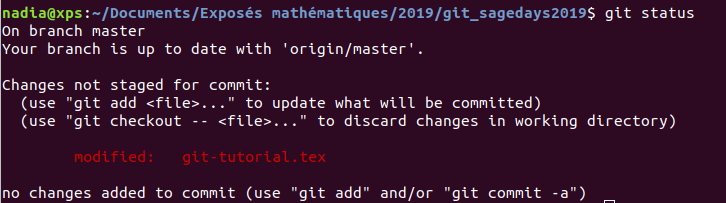
\includegraphics[width=\linewidth]{status}
		\end{center}
	\end{frame}

	\begin{frame}{First steps: Creating a folder + initializing}

	\end{frame}
	\begin{frame}[fragile]{Getting code: cloning}
	To get code from a remote repository:
	\begin{verbatim}
$ git clone https://address-of-the-repo.git
	\end{verbatim}
	Maybe some of you did, yesterday,
	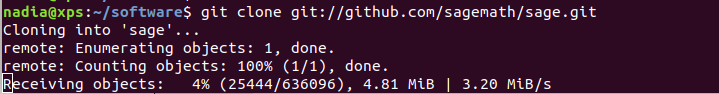
\includegraphics[width=\linewidth]{clone}
	\pause
	\begin{exo}
		Clone the repository containing this talk.
		\url{https://github.com/phubert/git_sagedays2019.git}
	\end{exo}
	\end{frame}
	\begin{frame}{Modifications}
		
	\end{frame}
	\begin{frame}{Sharing modifications}
		contenu...
	\end{frame}
	\begin{frame}{Getting updated code \& solving conflicts}
	
	\end{frame}
	\begin{frame}{Reviewing changes}
		You can look at what other people did:
		\begin{itemize}
			\item on a software\\
		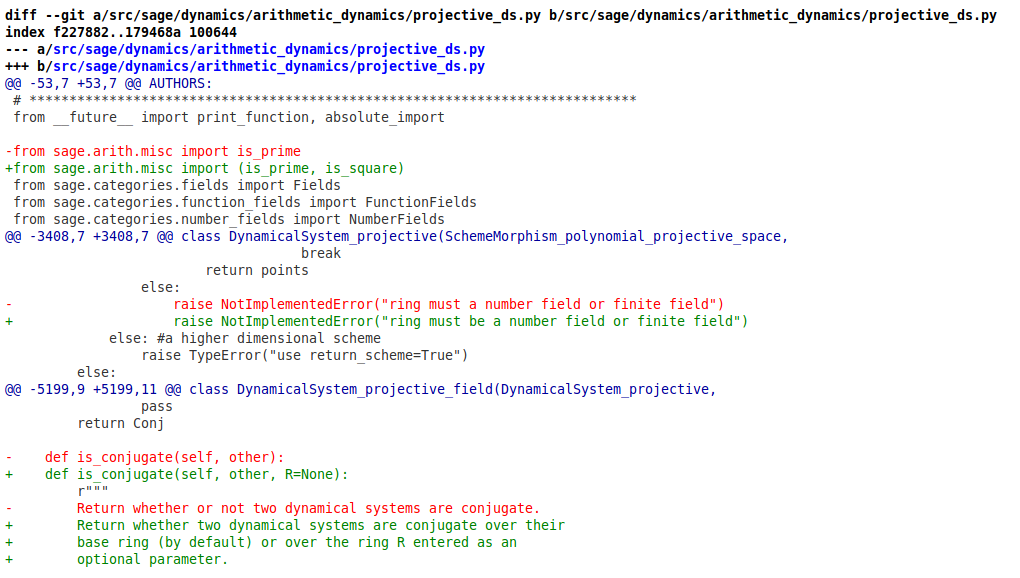
\includegraphics[width=0.8\linewidth]{diff_on_sage_2}  %ticket 28070
			\item on your files\\
		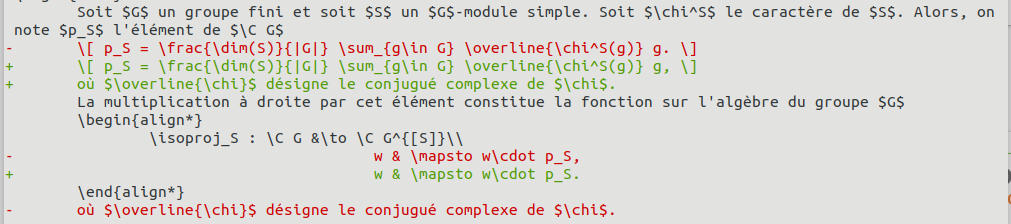
\includegraphics[width=0.8\linewidth]{diff_on_latex}
		\end{itemize}
	\end{frame}
	\begin{frame}[fragile]{Reviewing changes}
	To know what has been change since last commit:
	\begin{verbatim}
$ git diff
	\end{verbatim}
	or since commit1 
\begin{verbatim}
$ git diff commit1
\end{verbatim}
	or between commit1 and commit2
	\begin{verbatim}
$ git diff commit1 commit2
	\end{verbatim}
	\begin{tcolorbox}[colback=cyan!30]
		To recover the "name" of commit1, you must type \texttt{git log} (this is the history of the repository). The name is very long!\\
		(e.g.: df14e25763073c18e30ebeede3d34ef466dd08c8)
	\end{tcolorbox}
	\end{frame}
	\begin{frame}{Reviewing changes}
		You can do it with a graphical user interface (e.g. Meld 
\includegraphics[height=1em]{meld_logo}).\\
		\vspace{1em}
		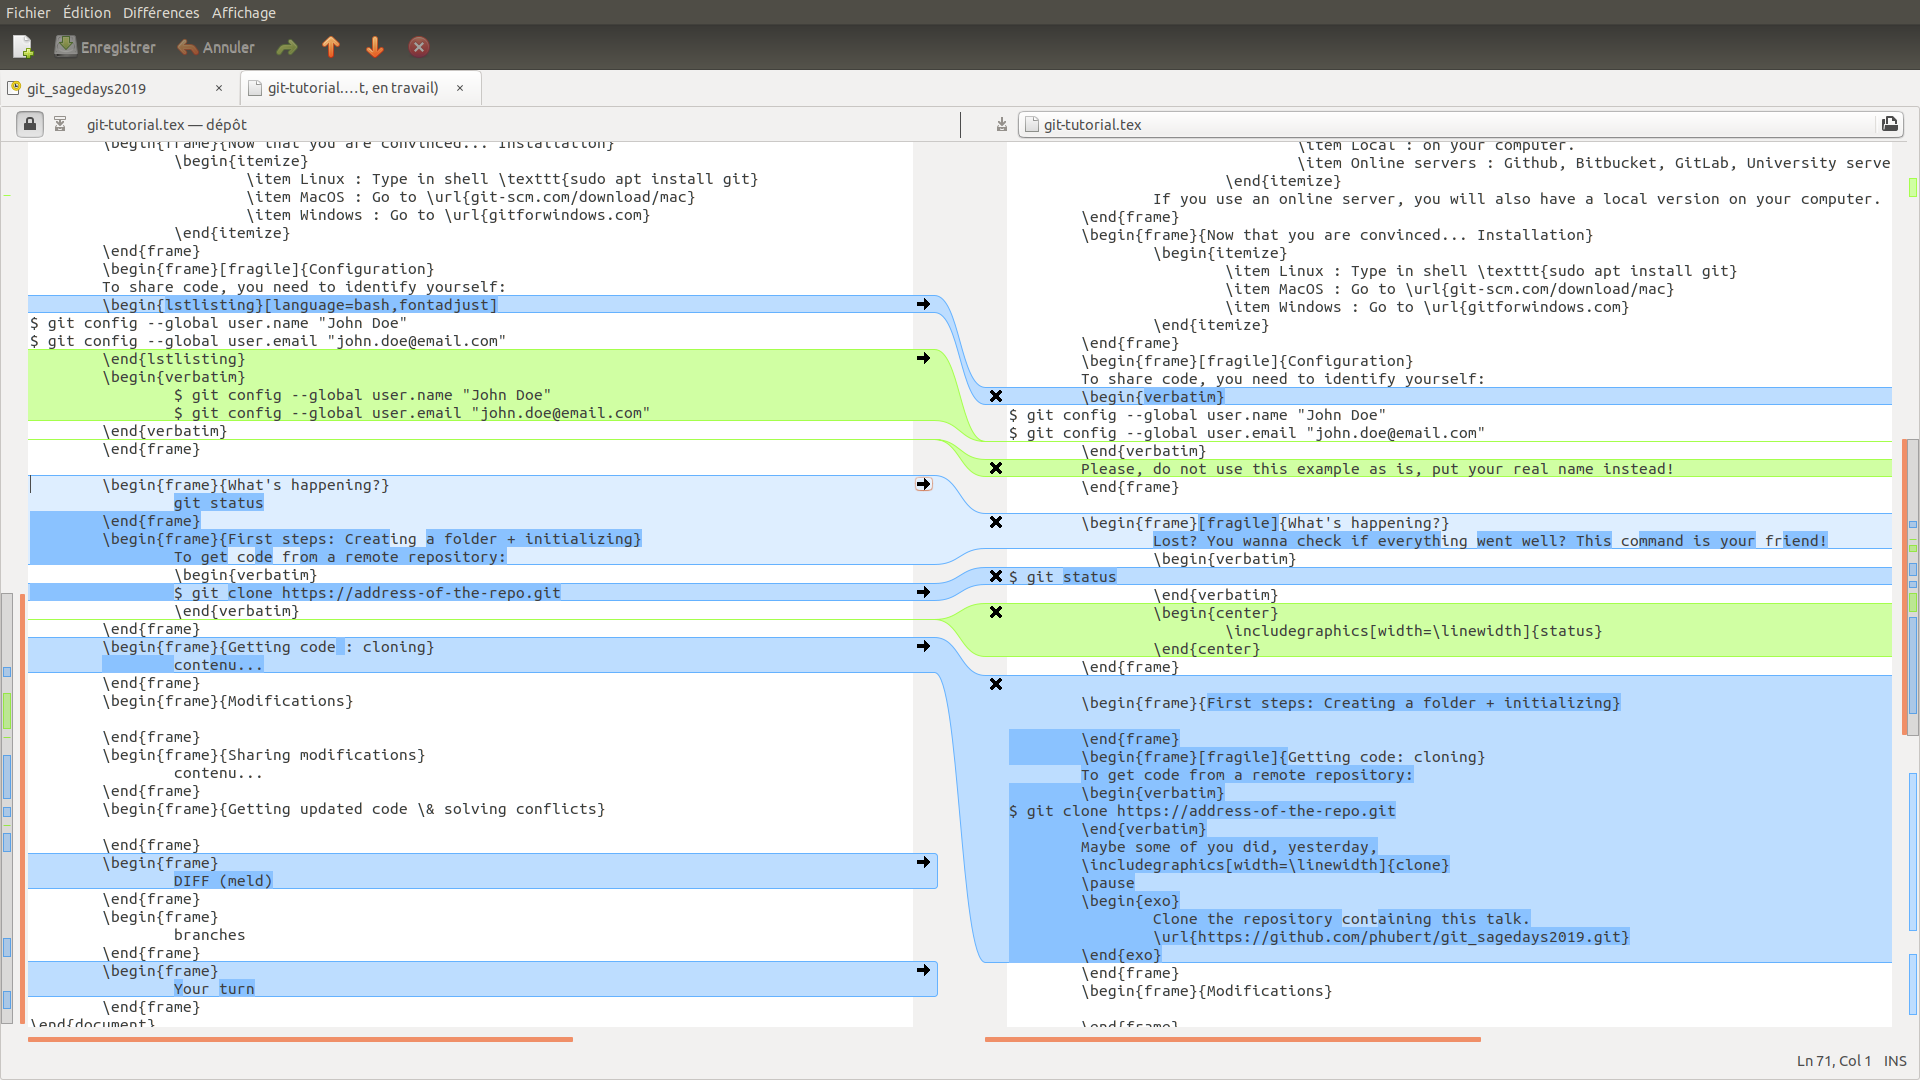
\includegraphics[width=\linewidth]{meld_ps}
	\end{frame}
	\begin{frame}
		branches
	\end{frame}
	\begin{frame}{Your turn!}
	Two-by-two, try the following:
		\begin{itemize}
			\item Get in the Exercise folder of our repository (you \textit{need} to clone the repository from \url{https://github.com/phubert/git_sagedays2019.git} ).
			\item Create your own branch (name it after the concatenation of your names).
			\item Edit three of the files.
			\item Send your files to the server. \textit{Don't forget to put a relevant commit message!}
			\item We will add mistakes in your files.
			\item Get the modifications and correct the mistakes. Send everything back to us.
		\end{itemize}
	\end{frame}
\end{document}